\documentclass[conference]{IEEEtran}
\IEEEoverridecommandlockouts
\usepackage{}
\usepackage{cite}
\usepackage{amsmath,amssymb,amsfonts}
\usepackage{algorithm}
\usepackage{algorithmic}
\usepackage{float}
\usepackage{graphicx}
\usepackage{textcomp}
\usepackage{xcolor}
\usepackage[colorlinks=true,allcolors=blue]{hyperref}
\usepackage{placeins}
\usepackage{subcaption}
\usepackage{fontawesome5}

\pagestyle{plain}

\def\BibTeX{{\rm B\kern-.05em{\sc i\kern-.025em b}\kern-.08em
    T\kern-.1667em\lower.7ex\hbox{E}\kern-.125emX}}

\begin{document}

\title{Autonomous UAV Localization via Aerial-to-Satellite Image Registration\thanks{Source code available on our \href{https://github.com/BohdanZasymovych/uav-image-to-map-localization}{\faGithub\ GitHub repository}}}

\author{
\IEEEauthorblockN{Solomiia Gadiichuk}
\IEEEauthorblockA{\textit{Faculty of Applied Sciences} \\
Ukrainian Catholic University\\
Lviv, Ukraine \\
hadiichuk.pn@ucu.edu.ua}
\and
\IEEEauthorblockN{Bohdan Zasymovych}
\IEEEauthorblockA{\textit{Faculty of Applied Sciences} \\
Ukrainian Catholic University\\
Lviv, Ukraine\\
zasymovych.pn@ucu.edu.ua}
\and
\IEEEauthorblockN{Marta Kosiv}
\IEEEauthorblockA{\textit{Faculty of Applied Sciences} \\
Ukrainian Catholic University\\
Lviv, Ukraine\\
kosiv.pn@ucu.edu.ua}
}

\maketitle

\begin{abstract}
Navigating Unmanned Aerial Vehicles (UAVs) in GNSS-denied environments is a critical challenge due to the massive deployment of Electronic Warfare systems. When satellite navigation fails, autonomous systems need reliable alternatives for absolute positioning. This project develops a vision-based localization engine that calculates a UAV's geographic coordinates by matching its real-time camera feed against preloaded satellite maps. The pipeline uses SIFT for feature extraction and RANSAC for geometric outlier rejection to estimate an Affine transformation between images. The estimated model then projects the drone's optical center onto the global coordinate plane.
\end{abstract}

\begin{IEEEkeywords}
UAV Localization, GNSS-denied Navigation, Image Registration, Feature Matching, Affine Transformation, RANSAC, SIFT
\end{IEEEkeywords}

\section{Introduction}

\subsection{Problem Context}
Visual Unmanned Aerial Vehicle (UAV) localization enables autonomous flight by calculating absolute geographic coordinates solely from optical sensors. This involves matching the UAV's real-time images against georeferenced satellite maps.

\begin{figure}[htbp]
    \centering
    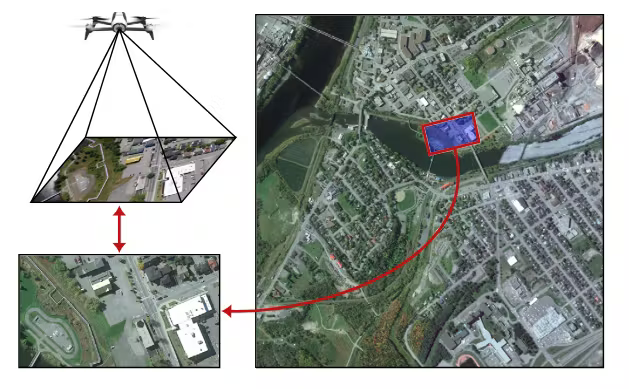
\includegraphics[width=1\columnwidth]{figs/image_to_map_localization.png}
    \caption{Matching the UAV camera feed to a reference satellite map \cite{b1}.}
    \label{fig:image_to_map}
\end{figure}

These systems are critical in modern warfare, where Electronic Warfare (EW) makes Global Navigation Satellite Systems (GNSS) highly vulnerable. Vision-based localization offers a passive, unjammable alternative, allowing UAVs to compute coordinates from onboard visual data and navigate GNSS-denied environments.

This project develops an automated vision-based positioning system for UAVs.

\section{Related Work}

\subsection{Absolute Visual Localization Approaches}
As outlined in \cite{b1}, vision-based localization includes map-independent methods (estimating relative motion with drift) and map-based methods (providing drift-free absolute coordinates). For map-based UAV-to-satellite registration, there are three primary paradigms:

\begin{itemize}
    \item \textbf{Direct Template Matching:} Slides the real-time image across the reference map to find the highest raw pixel correlation.
    \item \textbf{Feature-Point Matching:} Extracts distinct geometric interest points and matches their mathematical descriptors.
    \item \textbf{Deep Learning-Based Matching:} Uses neural networks to extract high-level semantic context.
\end{itemize}

Template matching compares raw pixels, making it fast but sensitive to scale and rotation. Feature matching extracts geometric keypoints, ensuring robustness against tilt and altitude changes. Deep learning evaluates semantic context, handling extreme variations at high computational costs.

\subsection{Keypoint Detection and Description}
Feature detection computes abstractions of image information. Based on \cite{b2}, the primary traditional algorithms are:

\begin{itemize}
    \item \textbf{SIFT:} Uses Difference of Gaussian for scale-space extrema estimation and descriptor generation. While computationally complex, it is highly robust against rotation and affine transformations.
    \item \textbf{SURF:} Approximates the Difference of Gaussian with box filters. It performs faster than SIFT while maintaining detection quality.
    \item \textbf{ORB:} A fusion of FAST and BRIEF. It is the fastest algorithm but more sensitive to certain transformations than SIFT.
\end{itemize}

While ORB is faster, SIFT achieves higher matching rates across most transformations, including intensity, rotation, shearing, and fisheye distortion \cite{b2}. SIFT is selected for this project due to this robustness.

\section{Mathematical Foundations}

\subsection{Problem Fomulation}
% TODO: write content

\subsection{Scale-Invariant Feature Detection and Matching}
To establish correspondences between the UAV imagery and the reference map, we utilize the Scale-Invariant Feature Transform (SIFT) algorithm, which represents keypoints as 128-dimensional continuous feature vectors. The similarity between a query descriptor $v$ and a train descriptor $u$ is determined using the Euclidean distance ($L_2$ norm) in the feature space:
$$d(v, u) = \sqrt{\sum_{k=1}^{128} (v_k - u_k)^2}$$
Due to the highly repetitive nature of aerial landscapes, direct nearest-neighbor matching is prone to false positives. To mathematically mitigate this, correspondences are filtered using Lowe's ratio test. For any given descriptor, let $d_1$ be the distance to its closest neighbor and $d_2$ be the distance to the second closest neighbor. A match is considered reliable and unique only if it satisfies the following inequality:
$$\frac{d_1}{d_2} < \tau$$
where $\tau$ is a predefined ratio threshold.

\subsection{Robust Estimation via RANSAC}

Given a set of noisy correspondences between UAV image points and map points,
\[
\mathcal{D} = \{(x_i, y_i) \leftrightarrow (X_i, Y_i)\}_{i=1}^{N},
\]
the goal is to estimate transformation parameters $\theta$ (affine model)
that are consistent with the largest subset of correct matches (inliers),
while rejecting incorrect correspondences (outliers).

\textbf{Reprojection Error Definition.}

Each correspondence induces a reprojection error under model $\theta$:
\[
d_i(\theta) = \left\| 
\begin{bmatrix} X_i \\ Y_i \end{bmatrix}
-
\hat{T}_\theta
\begin{bmatrix} x_i \\ y_i \\ 1 \end{bmatrix}
\right\|_2,
\]
where $\hat{T}_\theta$ is the affine transformation matrix.

A point is considered an inlier if:
\[
d_i(\theta) < \epsilon,
\]
where $\epsilon$ is a predefined threshold.

Thus, the objective is:
\[
\theta^* = \arg\max_{\theta} \sum_{i=1}^{N} \mathbf{1}\big(d_i(\theta) < \epsilon\big),
\]
i.e., maximize the number of inliers.

\textbf{RANSAC Iterative Procedure.}

At each iteration, a minimal subset of $s$ correspondences is sampled:
\[
\mathcal{S} \subset \mathcal{D}, \quad |\mathcal{S}| = s,
\]
where for the affine model $s = 3$.

Using this subset, a candidate model $\theta$ is estimated by solving
the linear system defined by the affine transformation.

The model is then evaluated on the full dataset by computing
the reprojection errors $\{d_i(\theta)\}_{i=1}^{N}$ and constructing
the inlier set:
\[
\mathcal{I}(\theta) = \{ i \mid d_i(\theta) < \epsilon \}.
\]

The model with the largest consensus set is selected:
\[
\theta^* = \arg\max_{\theta} |\mathcal{I}(\theta)|.
\]

\textbf{Adaptive Number of Iterations.}

The number of RANSAC iterations is derived probabilistically.
Let $w$ denote the probability that a randomly selected correspondence is an inlier:
\[
w = \frac{|\mathcal{I}|}{N}.
\]

The probability that all $s$ points in a randomly sampled subset are inliers is:
\[
P_{\text{all-inliers}} = w^s.
\]

Thus, the probability that a sampled subset contains at least one outlier is:
\[
1 - w^s.
\]

If we perform $k$ independent iterations, the probability that all sampled subsets
contain at least one outlier is:
\[
(1 - w^s)^k.
\]

Therefore, the probability that at least one of the $k$ samples consists entirely
of inliers is:
\[
1 - (1 - w^s)^k.
\]

To guarantee a desired confidence level $p$, we require:
\[
1 - (1 - w^s)^k \geq p.
\]

Rearranging the inequality:
\[
(1 - w^s)^k \leq 1 - p.
\]

Taking logarithms on both sides:
\[
k \log(1 - w^s) \leq \log(1 - p).
\]

Finally, solving for $k$:
\[
k = \frac{\log(1 - p)}{\log(1 - w^s)}.
\]

\textbf{Final Model Estimation.}

After identifying the best inlier set $\mathcal{I}^*$, the final model
parameters are recomputed using all inliers by solving the
overdetermined system:
\[
A v = b,
\]
using the least-squares solution:
\[
v = (A^T A)^{-1} A^T b.
\]



\subsection{Geometric Transformation Models}
Geometric transformations define the mathematical mapping between UAV imagery and the reference map. We consider three linear models:

\begin{itemize}
	\item \textbf{Similarity Transformation:} A 4-degree-of-freedom model accounting for translation, rotation, and uniform scaling.
	\item \textbf{Affine Transformation:} A 6-degree-of-freedom model extending similarity by adding shear and non-uniform scaling.
	\item \textbf{Projective:} An 8-degree-of-freedom model representing the true 3D to 2D projection.
\end{itemize}

The Similarity model requires perfectly level flight and uniform zooming, failing with axial stretching or tilt. The Affine model approximates slight perspective shifts via shear, but only the Projective model handles significant pitch and roll by modeling converging parallel lines.

We chose the Affine model because it flexibly handles non-ideal conditions (slight tilt or shearing) while remaining mathematically simpler and more stable than the Projective model.

For the selected Affine model, the mapping between UAV coordinates $(x, y)$ and map coordinates $(X, Y)$ is:
\begin{equation}
\begin{bmatrix} X \\ Y \\ 1 \end{bmatrix} =
\begin{bmatrix} a_1 & a_2 & t_x \\ a_3 & a_4 & t_y \\ 0 & 0 & 1 \end{bmatrix}
\begin{bmatrix} x \\ y \\ 1 \end{bmatrix}
\end{equation}

During robust fitting, candidate transformations are scored by reprojection error for each correspondence:
\begin{equation}
d = \sqrt{(X_i - \hat{X}_i)^2 + (Y_i - \hat{Y}_i)^2} < \epsilon
\end{equation}

Given the final set of $n$ inliers, parameters are re-estimated from the overdetermined linear system $A\mathbf{v} = \mathbf{b}$ with $\mathbf{v} = [a_1, a_2, t_x, a_3, a_4, t_y]^T$:
\begin{equation}
\begin{bmatrix}
x_1 & y_1 & 1 & 0 & 0 & 0 \\
0 & 0 & 0 & x_1 & y_1 & 1 \\
\vdots & \vdots & \vdots & \vdots & \vdots & \vdots \\
x_n & y_n & 1 & 0 & 0 & 0 \\
0 & 0 & 0 & x_n & y_n & 1
\end{bmatrix}
\begin{bmatrix} a_1 \\ a_2 \\ t_x \\ a_3 \\ a_4 \\ t_y \end{bmatrix} =
\begin{bmatrix} X_1 \\ Y_1 \\ \vdots \\ X_n \\ Y_n \end{bmatrix}
\end{equation}

\subsection{Least-Squares Parameter Estimation}
The optimal solution $\mathbf{v}_{final}$ is the one that minimizes the sum of squared residuals, defined by the cost function $J(\mathbf{v})$:
\begin{equation}
J(\mathbf{v}) = \|A\mathbf{v} - \mathbf{b}\|^2 = (A\mathbf{v} - \mathbf{b})^T(A\mathbf{v} - \mathbf{b})
\end{equation}

Expanding the terms, we obtain:
\begin{equation}
J(\mathbf{v}) = \mathbf{v}^T A^T A \mathbf{v} - 2\mathbf{b}^T A \mathbf{v} + \mathbf{b}^T \mathbf{b}
\end{equation}

To find the minimum, we compute the derivative with respect to $\mathbf{v}$ and set it to zero:
\begin{equation}
\frac{\partial J(\mathbf{v})}{\partial \mathbf{v}} = 2A^T A \mathbf{v} - 2A^T \mathbf{b} = 0
\end{equation}

Solving this linear equation yields the final parameter vector:
\begin{equation}
A^T A \mathbf{v} = A^T \mathbf{b} \implies \mathbf{v}_{final} = (A^T A)^{-1} A^T \mathbf{b}
\end{equation}

\section{Localization Pipeline}\label{sec:localization_pipeline}

\subsection{Feature Extraction and Matching}\label{subsec:pipeline_feature_extraction}
The feature extraction module accepts two raw BGR images (the UAV camera feed and the reference satellite map) as input, explicitly converting them to grayscale prior to processing. First, SIFT keypoints and descriptors are computed for both images. Second, to bypass the $\mathcal{O}(N \cdot M)$ computational bottleneck of Brute-Force matching, we implement the Fast Library for Approximate Nearest Neighbors (FLANN). By structuring the satellite map descriptors into a randomized KD-tree forest (configured with 5 trees and 50 search checks), the matching complexity is reduced to $\mathcal{O}(N \log M)$, enabling rapid nearest-neighbor retrieval.  These initial matches are subsequently filtered using Lowe's ratio test (as defined in \autoref{subsec:feature_detection}) with a threshold of $\tau = 0.75$. This specific threshold is chosen to eliminate the vast majority of ambiguous matches caused by repetitive textures while retaining a sufficient number of high-quality geometric anchors. The final output of this stage consists of two corresponding arrays, \texttt{src\_pts} and \texttt{dst\_pts}, each of shape $(N, 2)$, which represent the matched pixel coordinates in the UAV and map coordinate spaces, respectively.

\subsection{RANSAC Configuration}\label{subsec:pipeline_ransac}
The RANSAC algorithm is applied to the set of matched feature correspondences to robustly estimate the transformation by filtering out outliers within the overall pipeline. We use an inlier threshold $\epsilon = 3$ pixels, meaning that a correspondence is considered consistent with the model if its reprojection error is below this value, as defined in \autoref{subsec:ransac}; smaller values may reject valid matches due to noise, while larger values may include outliers and degrade accuracy. The confidence parameter is set to $p = 0.99$, ensuring a high probability of sampling at least one all-inlier subset according to the probabilistic model described in \autoref{subsec:ransac}, while the number of iterations is capped at $2000$ to limit computation time in worst-case scenarios. The minimal sample size $s$ depends on the chosen transformation model (e.g., $s = 3$ for Affine, $s = 4$ for Projective), which directly affects the required number of iterations $k$; larger minimal sets lead to slower convergence but allow modeling more complex perspective transformations. The output of this stage is a boolean inlier mask over all correspondences, identifying geometrically consistent matches.

\subsection{Transformation Estimation}\label{subsec:pipeline_estimation}
This stage uses the inlier mask returned by RANSAC and discards all rejected correspondences. For the selected model (Similarity, Affine, or Projective), the pipeline instantiates the appropriate mathematical system defined in \autoref{subsec:transformation_models}. Linear models are solved via the least-squares method, while the Projective model applies Hartley's data normalization and solves the Direct Linear Transformation (DLT) using Singular Value Decomposition (SVD), as detailed in \autoref{subsec:parameter_estimation}. The output of this stage is the final estimated $3 \times 3$ transformation matrix $M$, which is consumed by the coordinate projection step.

\subsection{Coordinate Projection}\label{subsec:pipeline_projection}
The estimated matrix $M$ is applied to the UAV-image center in homogeneous coordinates, where $W$ and $H$ are the UAV image width and height:
\begin{equation}
\mathbf{c}_{uav} =
\begin{bmatrix}
W/2 \\
H/2 \\
1
\end{bmatrix}
\end{equation}

The matrix multiplication yields the projected coordinates and the homogeneous scale factor $W'$:
\begin{equation}
\begin{bmatrix}
\tilde{X} \\
\tilde{Y} \\
W'
\end{bmatrix}
= M\mathbf{c}_{uav}
\end{equation}

Finally, perspective division is applied to recover the true 2D Cartesian coordinates on the global map: 
\begin{equation}
(X_{map}, Y_{map}) = \left(\frac{\tilde{X}}{W'}, \frac{\tilde{Y}}{W'}\right).
\end{equation}

\subsection{Complete Pipeline}\label{subsec:pipeline_complete}
\begin{algorithm}[H]
\caption{UAV Localization Pipeline}
\begin{algorithmic}[1]
\REQUIRE UAV Image $I_{uav}$, Reference Map $I_{map}$
\ENSURE Global Coordinates $(X_{map}, Y_{map})$
\STATE Convert $I_{uav}$ and $I_{map}$ to grayscale.
\STATE Extract SIFT features and match using Lowe's ratio test.
\STATE \textbf{while} $i < \text{max\_iterations}$ \textbf{do}
\STATE \quad Sample minimal correspondence set $s$ and compute $M_{\text{temp}}$.
\STATE \quad Count inliers satisfying reprojection error $d < \epsilon$.
\STATE \quad If current consensus is the largest, store $M_{\text{temp}}$ and inlier mask.
\STATE \textbf{end while}
\STATE Compute optimal transformation $M$ using the full inlier set.
\STATE Project UAV center $(x_c, y_c, 1)^\top$ through $M$.
\STATE Apply perspective division to obtain $(X_{map}, Y_{map})$.
\RETURN $(X_{map}, Y_{map})$
\end{algorithmic}
\end{algorithm}
\section{Evaluation Strategy}

To ensure a robust and comprehensive assessment of the localization pipeline, we utilize a two-tiered evaluation strategy. This approach combines controlled synthetic experiments with large-scale validation on real-world aerial data.

\subsection{Synthetic Dataset}
The synthetic dataset is used for controlled and reproducible validation of the mathematical transformation models. Each test frame is created by sampling a high-resolution satellite orthophoto patch and applying a known affine deformation around its center. The transformed patch is treated as a synthetic UAV frame, while the center of the original sampled patch provides an absolute ground truth in map pixel coordinates.

For evaluation, we generate $N$ frames and run the localization pipeline independently on each. Frames that fail due to insufficient correspondences or model estimation errors are logged and excluded from accuracy statistics but included in success rate calculations.

\subsection{Real Dataset}
To validate the system's performance under actual flight conditions, we utilize the \textbf{UAV-VisLoc} dataset \cite{uav_visloc}. UAV-VisLoc is a large-scale benchmark specifically designed for visual localization in GNSS-denied environments. It contains:
\begin{itemize}
    \item \textbf{6,742 UAV images} captured from both multi-rotor and fixed-wing drones at varying altitudes and heading angles.
    \item \textbf{11 orthorectified satellite maps} covering diverse terrains across 11 cities, including urban, rural, and hilly environments.
    \item \textbf{Comprehensive Metadata}, providing ground-truth GPS coordinates (latitude/longitude), shooting height, and drone pose for every image.
\end{itemize}
Matching UAV frames against these maps presents a significant "domain gap" challenge due to differences in sensors, lighting, and seasonal variations between the drone imagery and the satellite reference.

\subsection{Evaluated Metrics}
To quantify the performance of each model, we use the following metrics:

\begin{itemize}
    \item \textbf{Success Rate:} Defined as a \textit{Technical Success}, where the pipeline successfully extracts features, matches them, and produces a final coordinate through the RANSAC algorithm. This metric measures the reliability of the software execution and the existence of a geometric solution, regardless of its accuracy.
    \item \textbf{Root Mean Square Error (RMSE):} Measures the Euclidean localization error in map pixels:
\end{itemize}

\begin{equation}
e_i = \sqrt{(X_i - \hat{X}_i)^2 + (Y_i - \hat{Y}_i)^2},
\end{equation}
\begin{equation}
RMSE = \sqrt{\frac{1}{N}\sum_{i=1}^{N} e_i^2}.
\end{equation}

To characterize efficiency, we report runtime mean and standard deviation:
\begin{equation}
\mu_t = \frac{1}{N}\sum_{i=1}^{N} t_i, \qquad
\sigma_t = \sqrt{\frac{1}{N}\sum_{i=1}^{N}(t_i - \mu_t)^2}.
\end{equation}

To characterize geometric consistency and matching health, we use the mean inlier ratio:
\begin{equation}
r_i = \frac{n_i^{\text{inliers}}}{n_i^{\text{matches}}}, \qquad
\bar{r} = \frac{1}{N}\sum_{i=1}^{N} r_i,
\end{equation}
where $n_i^{\text{matches}}$ is the count of matches after Lowe's ratio test and $n_i^{\text{inliers}}$ is the count of points retained by RANSAC. Together, these metrics provide evidence of localization accuracy, computational cost, and the robustness of correspondence filtering.

\section{Results}\label{sec:results}

\subsection{Application Interface and Features}
To drive the localization engine, we implemented a comprehensive software suite consisting of a Command Line Interface (CLI) and an interactive Graphical User Interface (UI). These applications facilitate the end-to-end pipeline, from image ingestion to coordinate projection. Key features include:

\begin{itemize}
    \item \textbf{Model Versatility:} Full support for Similarity (4-DOF), Affine (6-DOF), and Projective (8-DOF) transformation models.
    \item \textbf{Algorithmic Tuning:} Real-time configuration of SIFT feature limits, Lowe's ratio, and adaptive RANSAC parameters (epsilon, confidence).
    \item \textbf{Rich Visualization:} Dynamic rendering of keypoint correspondences and projected UAV bounding boxes on the reference map.
    \item \textbf{Artifact Exporting:} Standardized reporting via JSON summaries and ZIP archives for batch processing.
\end{itemize}

\begin{figure}[H]
    \centering
    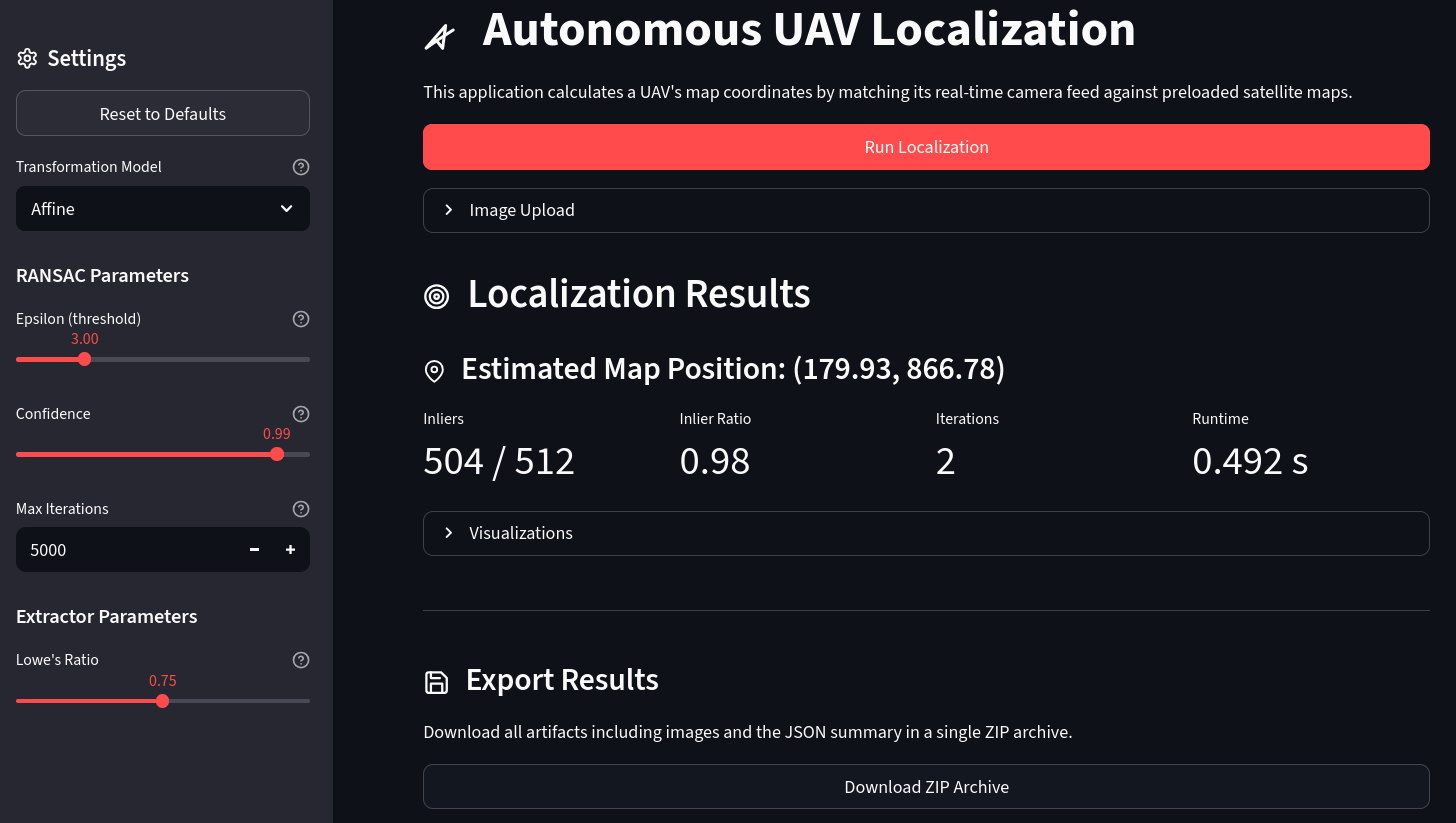
\includegraphics[width=1\columnwidth]{figs/app_ui.png}
    \caption{User Interface for the UAV Localization Application showing successful localization on a synthetic sample.}
    \label{fig:app_ui}
\end{figure}

\subsection{Single Image Match}\label{subsec:single_image_match}
Initial verification was conducted using a single simulated UAV frame. Using an Affine transformation model, the pipeline successfully matched 471 inliers from 478 raw matches ($98.5\%$ inlier ratio). The UAV center was estimated at $(179.99, 866.84)$ pixels in approximately $1.045$ seconds. Visual validation of the correspondences (\autoref{fig:matches_after_ransac}) and the final bounding box (\autoref{fig:map_with_bbox}) confirmed the mathematical correctness of the pipeline under ideal, noise-free conditions.

\begin{figure}[H]
    \centering
    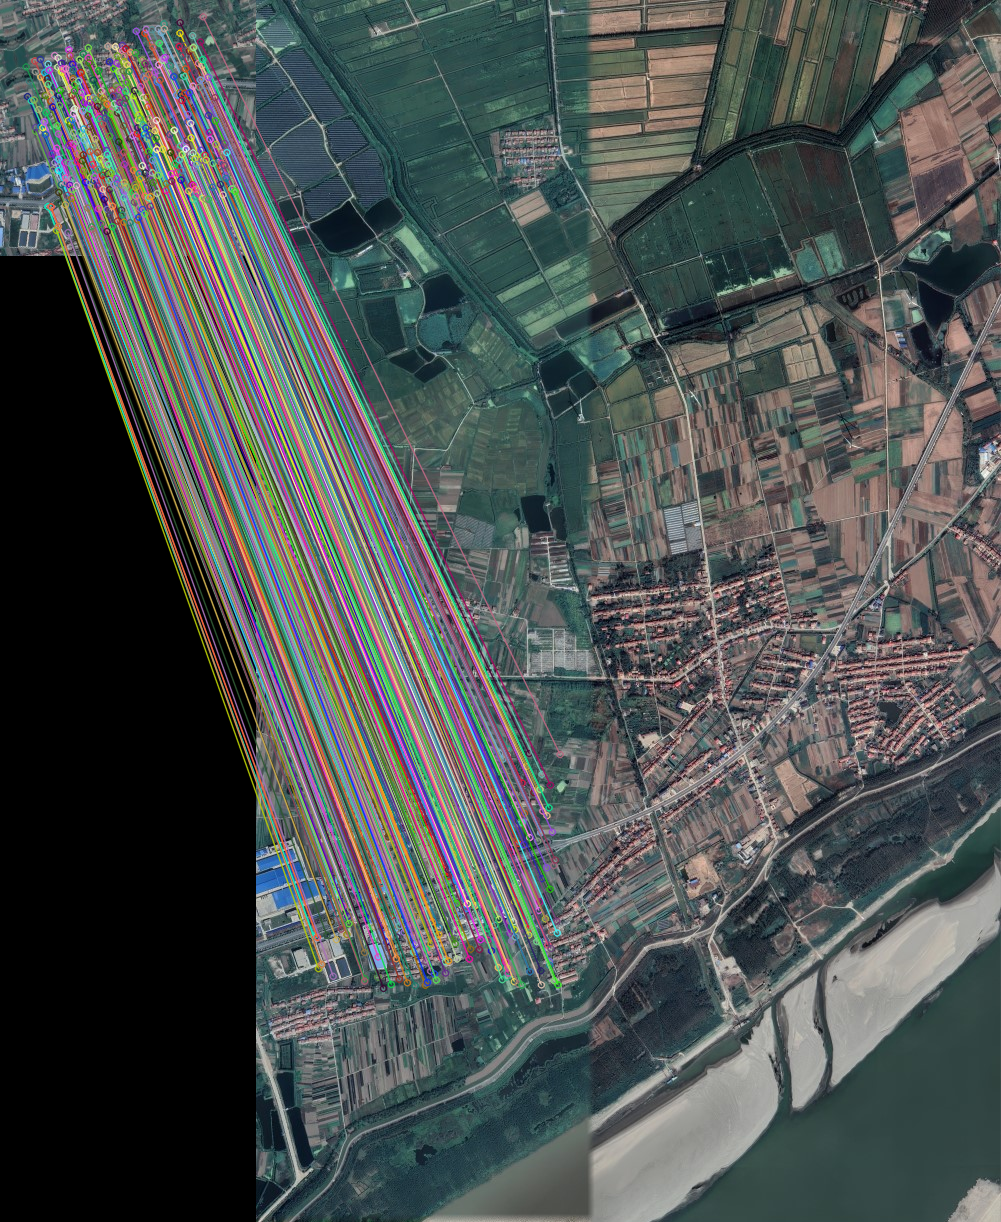
\includegraphics[width=1\columnwidth]{figs/matches_after_ransac.png}
    \caption{Geometrically consistent inlier matches retained after RANSAC filtering.}
    \label{fig:matches_after_ransac}
\end{figure}

\begin{figure}[H]
     \centering
     \begin{subfigure}[b]{0.6\columnwidth}
         \centering
         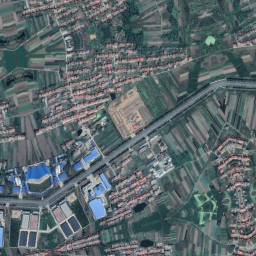
\includegraphics[width=\textwidth]{figs/uav_image.png}
         \caption{Input synthetic UAV frame.}
         \label{fig:uav_frame}
     \end{subfigure}
     \hfill
     \begin{subfigure}[b]{1.0\columnwidth}
         \centering
         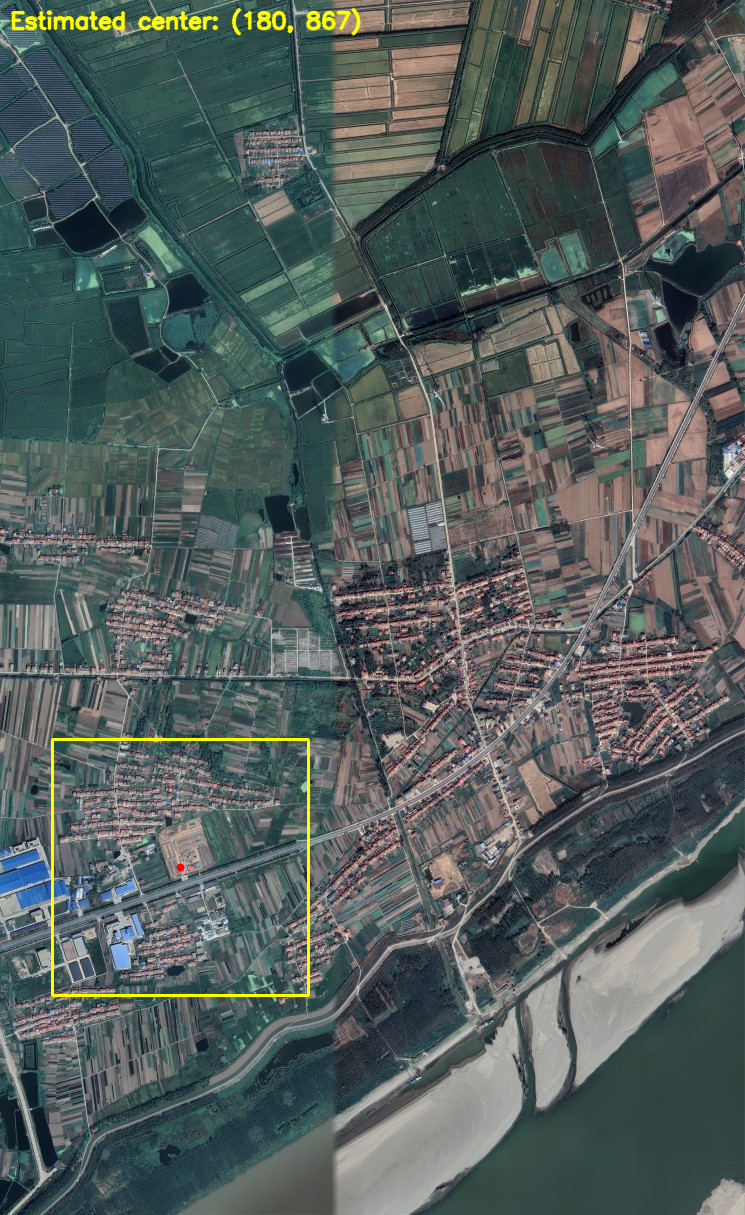
\includegraphics[width=\textwidth]{figs/map_with_estimated_bbox.png}
         \caption{Reference map with the projected UAV footprint.}
         \label{fig:map_footprint}
     \end{subfigure}
        \caption{Single image localization results showing the relationship between the captured frame and the global map.}
        \label{fig:map_with_bbox}
\end{figure}

\subsection{Synthetic Dataset Evaluation}\label{subsec:dataset_evaluation}
We benchmarked the pipeline on a controlled dataset of 60 synthetically deformed satellite crops. The system achieved a $90\%$ technical success rate with a mean RMSE of $16.69$ pixels. The distribution of errors (\autoref{fig:error_distribution}) confirms that the pipeline is highly precise when the UAV image is a direct geometric transformation of the reference map. 

\begin{figure}[H]
    \centering
    
\includegraphics[width=1\columnwidth]{figs/error_distribution.png}
    \caption{Distribution of localization errors across the synthetic dataset.}\label{fig:error_distribution}
\end{figure}

\subsection{Real Dataset Evaluation}\label{subsec:real_evaluation}
The final phase evaluated the pipeline on the UAV-VisLoc dataset \cite{uav_visloc} to compare the Similarity, Affine, and Projective models under real-world conditions. While all models achieved a $84\%$ technical success rate, the accuracy metrics diverged significantly.

\begin{table}[H]
    \caption{Comparative Performance Summary on the UAV-VisLoc Dataset.}\label{tab:real_results}
    \centering
    \begin{tabular}{|l|c|c|c|c|}
        \hline
        \textbf{Model} & \textbf{Success Rate} & \textbf{RMSE (px)} & \textbf{Inlier Ratio} & \textbf{Runtime (s)} \\
        \hline
        Similarity & 84\% & 45,713 & 0.079 & 1.90 \\
        Affine     & 84\% & 146,846 & 0.089 & 1.96 \\
        Projective & 84\% & 15,390 & 0.120 & 2.36 \\
        \hline
    \end{tabular}
\end{table}

\begin{figure}[H]
    \centering
    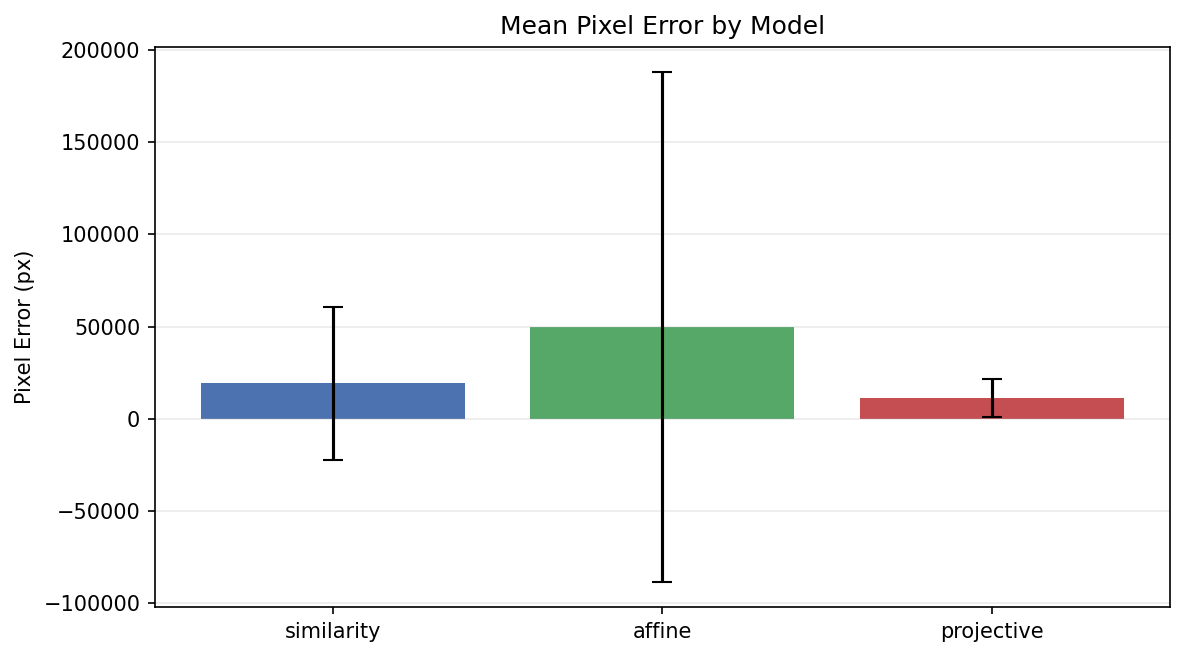
\includegraphics[width=1\columnwidth]{figs/pixel_error_by_model.png}
    \caption{Mean pixel error and standard deviation by transformation model.}
    \label{fig:real_pixel_error}
\end{figure}

The benchmark results (\autoref{tab:real_results}, \autoref{fig:real_pixel_error}) reveal a catastrophic degradation in accuracy compared to the synthetic tests. The Similarity and Affine models exhibited extreme Root Mean Square Errors, whereas the Projective model remained relatively more stable ($15,390$ px). The mean inlier ratio across all models dropped below $0.12$, indicating that over $88\%$ of SIFT correspondences were rejected as outliers. Furthermore, the Projective model exhibited a slightly higher runtime due to the computational overhead of Singular Value Decomposition (SVD) compared to the Normal Equations solver used for the other models.


\section{Conclusion and Future Outlook}\label{sec:conclusion}

The development and evaluation of this UAV localization engine have provided critical insights into the challenges of vision-based absolute positioning. Our experiments reveal a stark contrast between theoretical stability and real-world robustness.

\subsection{Summary of Findings}
The localization pipeline achieved high precision on the synthetic dataset ($90\%$ success, $16.69$px RMSE), proving that the core mathematical logic for coordinate projection and RANSAC-based estimation is sound. however, the transition to real-world data from the UAV-VisLoc benchmark exposed fundamental limitations. While the system remained technically functional, the localization error increased by several orders of magnitude.

\subsection{The Domain Gap Challenge}
The primary cause of the accuracy degradation is the "domain gap" between the UAV camera feed and georeferenced satellite maps. In real-world environments, the images are not merely geometric transformations of each other. Dynamic changes---such as seasonal variations, building renovations, moving vehicles, and differing sun angles---alter the local pixel gradients. Since SIFT relies on these gradients for feature description, the resulting correspondences were dominated by outliers, leading to the observed inlier ratios of less than $12\%$.

\subsection{Possible improvments}
To bridge this gap and achieve production-ready robustness, the pipeline must evolve beyond classical point-matching. Future development should focus on three tiers:

\begin{itemize}
    \item \textbf{Learned Matching:} Replace hand-crafted descriptors like SIFT with deep-learned feature extractors such as \textit{SuperPoint} or \textit{LoFTR}. These networks are trained to find invariant anchors across multi-modal aerial imagery, providing superior matching robustness compared to classical gradient-based methods \cite{opencv_matching}.
    \item \textbf{Semantic Registration:} Utilize semantic-guided feature detection to match high-level geometric structures (roads, intersections, building footprints) instead of raw textures \cite{xue2023sfd2}. This approach is naturally robust to seasonal and lighting changes as it prioritizes static urban features over transient visual patterns.
    \item \textbf{Hierarchical Search:} Implement a coarse-to-fine localization strategy.
 By using low-resolution global descriptors (e.g., \textit{NetVLAD}) to identify the general candidate area on the map, the search space for geometric matching is drastically reduced, decreasing the probability of false matches and improving computational efficiency.
\end{itemize}

In conclusion, while a classical SIFT-RANSAC architecture provides a strong foundation for controlled environments, autonomous UAV operation in unconstrained real-world settings requires a multi-modal approach combining geometry with high-level semantic understanding.

The complete source code are available on our \href{https://github.com/BohdanZasymovych/uav-image-to-map-localization}{\faGithub\ GitHub repository}.


\bibliographystyle{IEEEtran}
\bibliography{references}

\end{document}
